\documentclass[12pt,letterpaper]{article}
\usepackage{graphicx,textcomp}
\usepackage{natbib}
\usepackage{setspace}
\usepackage{fullpage}
\usepackage{color}
\usepackage[reqno]{amsmath}
\usepackage{amsthm}
\usepackage{fancyvrb}
\usepackage{amssymb,enumerate}
\usepackage[all]{xy}
\usepackage{endnotes}
\usepackage{lscape}
\newtheorem{com}{Comment}
\usepackage{float}
\usepackage{hyperref}
\newtheorem{lem} {Lemma}
\newtheorem{prop}{Proposition}
\newtheorem{thm}{Theorem}
\newtheorem{defn}{Definition}
\newtheorem{cor}{Corollary}
\newtheorem{obs}{Observation}
\usepackage[compact]{titlesec}
\usepackage{dcolumn}
\usepackage{tikz}
\usetikzlibrary{arrows}
\usepackage{multirow}
\usepackage{xcolor}
\newcolumntype{.}{D{.}{.}{-1}}
\newcolumntype{d}[1]{D{.}{.}{#1}}
\definecolor{light-gray}{gray}{0.65}
\usepackage{url}
\usepackage{listings}
\usepackage{color}

\definecolor{codegreen}{rgb}{0,0.6,0}
\definecolor{codegray}{rgb}{0.5,0.5,0.5}
\definecolor{codepurple}{rgb}{0.58,0,0.82}
\definecolor{backcolour}{rgb}{0.95,0.95,0.92}

\lstdefinestyle{mystyle}{
	backgroundcolor=\color{backcolour},   
	commentstyle=\color{codegreen},
	keywordstyle=\color{magenta},
	numberstyle=\tiny\color{codegray},
	stringstyle=\color{codepurple},
	basicstyle=\footnotesize,
	breakatwhitespace=false,         
	breaklines=true,                 
	captionpos=b,                    
	keepspaces=true,                 
	numbers=left,                    
	numbersep=5pt,                  
	showspaces=false,                
	showstringspaces=false,
	showtabs=false,                  
	tabsize=2
}
\lstset{style=mystyle}
\newcommand{\Sref}[1]{Section~\ref{#1}}
\newtheorem{hyp}{Hypothesis}

\title{Problem Set 1}
\date{Due: September 30, 2024}
\author{Applied Stats/Quant Methods 1}

\begin{document}
	\maketitle
	
	\section*{Instructions}
	\begin{itemize}
	\item Please show your work! You may lose points by simply writing in the answer. If the problem requires you to execute commands in \texttt{R}, please include the code you used to get your answers. Please also include the \texttt{.R} file that contains your code. If you are not sure if work needs to be shown for a particular problem, please ask.
\item Your homework should be submitted electronically on GitHub.
\item This problem set is due before 23:59 on Monday September 30, 2024. No late assignments will be accepted.
%\item Total available points for this homework is 80.
	\end{itemize}
	
	\vspace{1cm}
	\section*{Question 1: Education}

A school counselor was curious about the average of IQ of the students in her school and took a random sample of 25 students' IQ scores. The following is the data set:\\

\begin{enumerate}
	\item Find a 90\% confidence interval for the average student IQ in the school.
   \lstinputlisting[language=R, firstline=35, lastline=61]{PS01.R}  
	\item Next, the school counselor was curious  whether  the average student IQ in her school is higher than the average IQ score (100) among all the schools in the country.\\ 
	\noindent Using the same sample, conduct the appropriate hypothesis test with $\alpha=0.05$.
		\lstinputlisting[language=R, firstline=64, lastline=82]{PS01.R}  
\end{enumerate}
      The average IQ of students in her school is higher than the average IQ\\
\newpage

\part{title}	\section*{Question 2: Political Economy}

\noindent Researchers are curious about what affects the amount of money communities spend on addressing homelessness. The following variables constitute our data set about social welfare expenditures in the USA. \\
\vspace{.5cm}


\begin{tabular}{r|l}
	\texttt{State} &\emph{50 states in US} \\
	\texttt{Y} & \emph{per capita expenditure on shelters/housing assistance in state}\\
	\texttt{X1} &\emph{per capita personal income in state} \\
	\texttt{X2} &  \emph{Number of residents per 100,000 that are "financially insecure" in state}\\
	\texttt{X3} &  \emph{Number of people per thousand residing in urban areas in state} \\
	\texttt{Region} &  \emph{1=Northeast, 2= North Central, 3= South, 4=West} \\
\end{tabular}

\vspace{.5cm}
\noindent Explore the \texttt{expenditure} data set and import data into \texttt{R}.
\begin{itemize}
\item
Please plot the relationships among \emph{Y}, \emph{X1}, \emph{X2}, and \emph{X3}? What are the correlations among them (you just need to describe the graph and the relationships among them)?
\lstinputlisting[language=R, firstline=88, lastline=119]{PS01.R}  

\begin{figure}[h!]\centering
	\caption{\footnotesize scatter Matrix}
	\label{fig:1}
	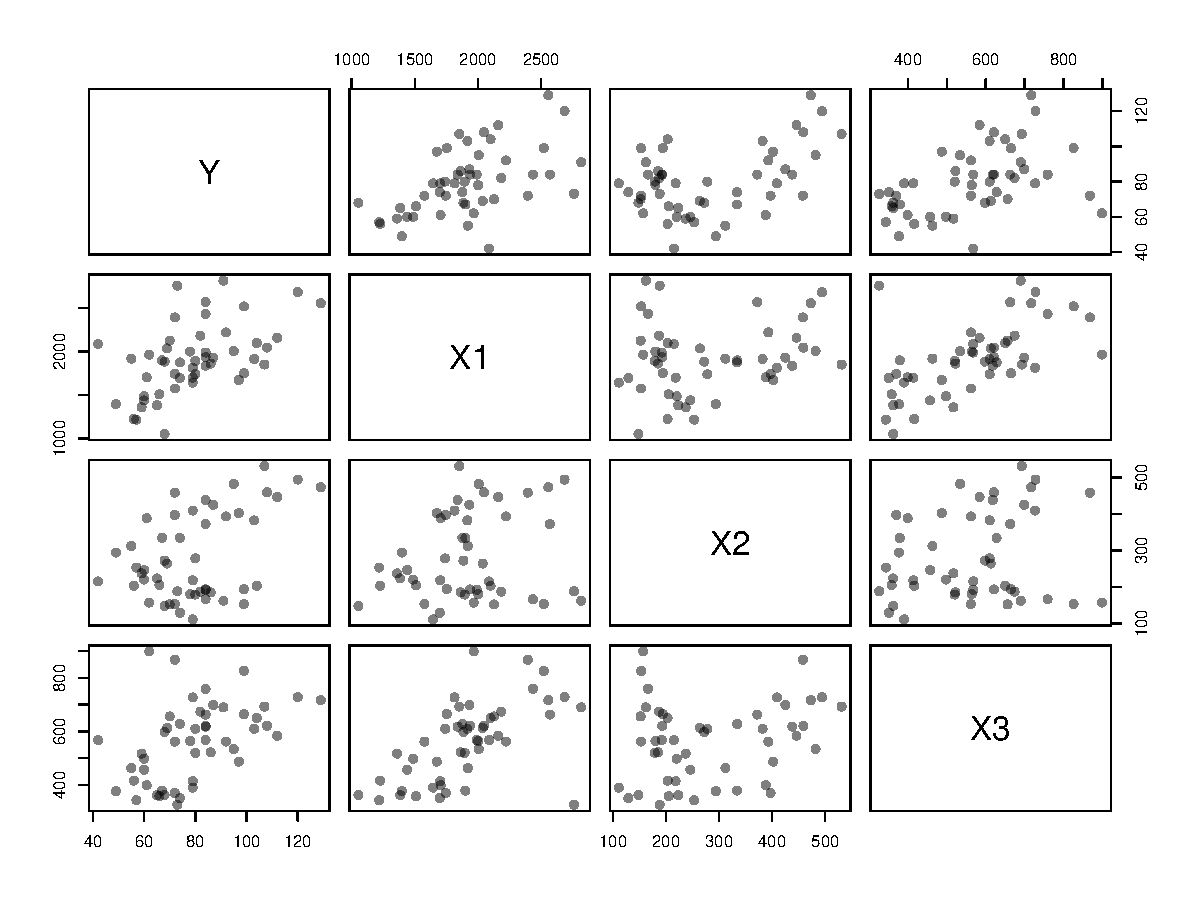
\includegraphics[width=.75\textwidth]{scatter_Matrix.pdf}
\end{figure}

 \begin{figure}[h!]\centering
	\caption{\footnotesize Y X1}
	\label{fig:3}
	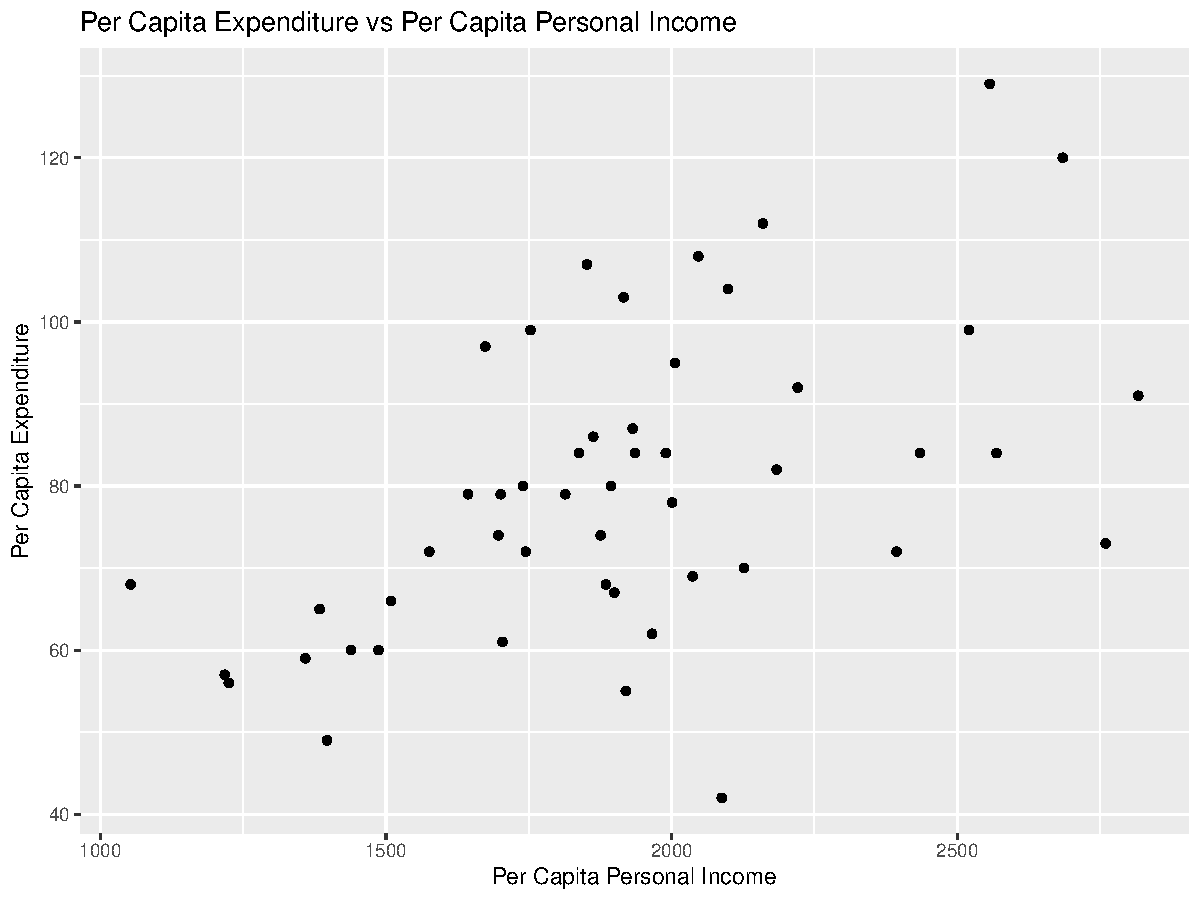
\includegraphics[width=.75\textwidth]{Y_vs_X1.pdf}
\end{figure}

 \begin{figure}[h!]\centering
	\caption{\footnotesize X2 Y}
	\label{fig:5}
	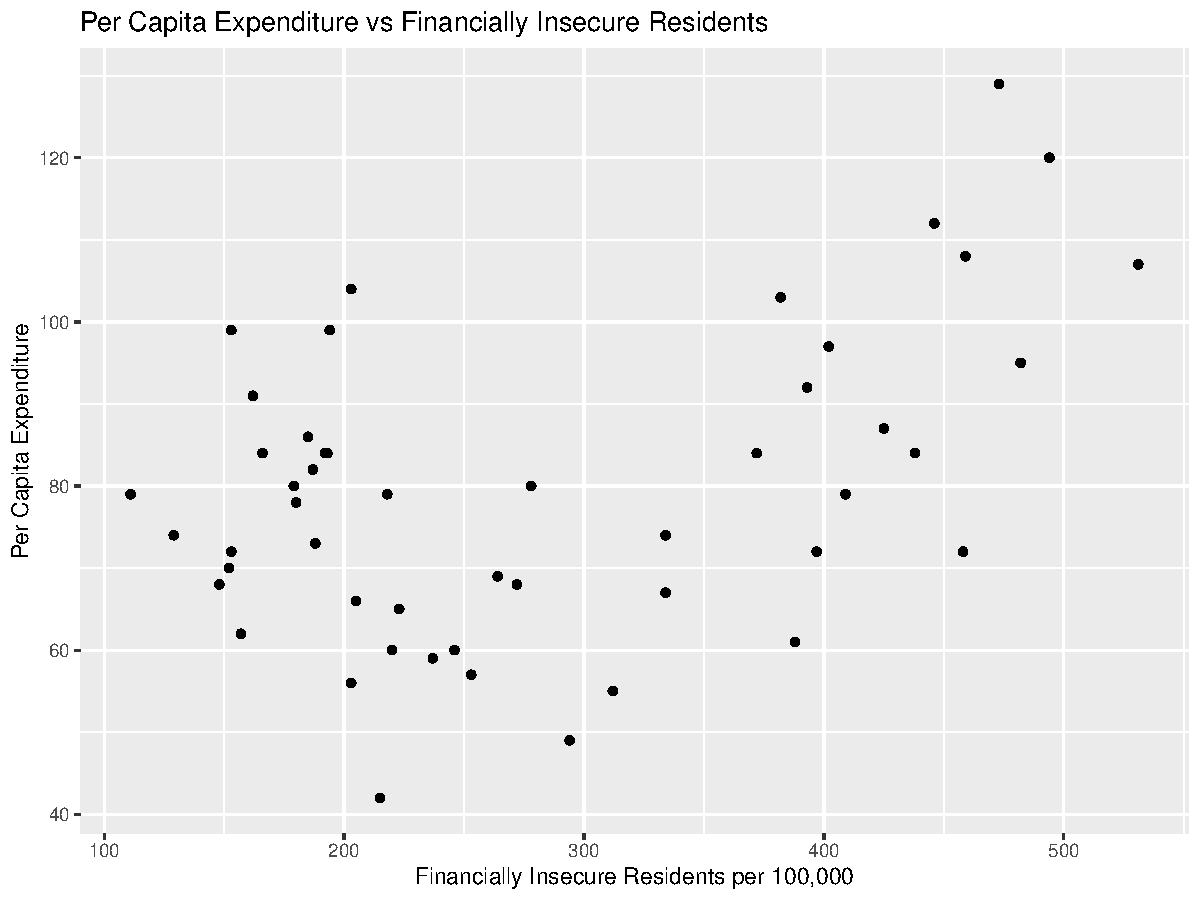
\includegraphics[width=.75\textwidth]{X2_Y.pdf}
\end{figure}

\begin{figure}[h!]\centering
	\caption{\footnotesize X3 Y}
	\label{fig:6}
	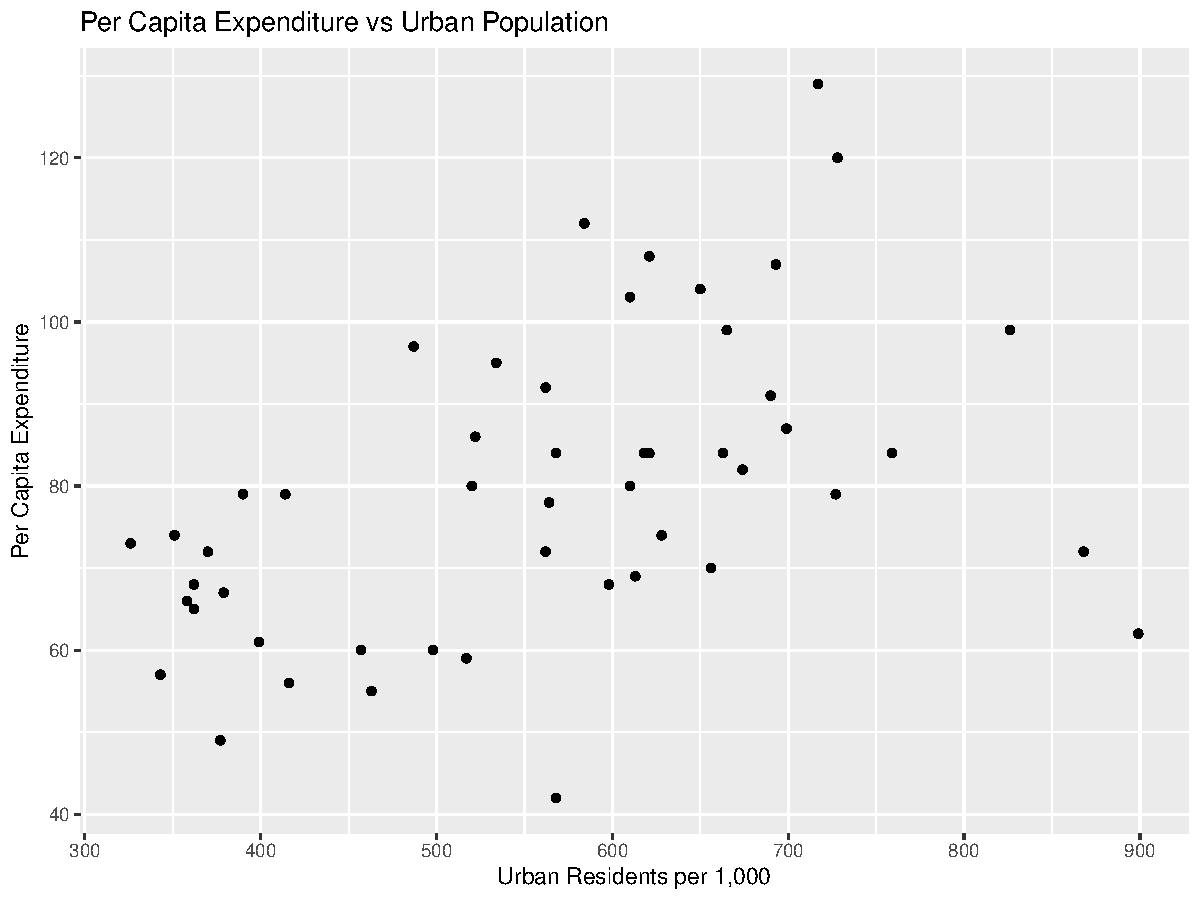
\includegraphics[width=.75\textwidth]{X3_Y.pdf}
\end{figure}

\begin{figure}[h!]\centering
	\caption{\footnotesize X1 X2}
	\label{fig:7}
	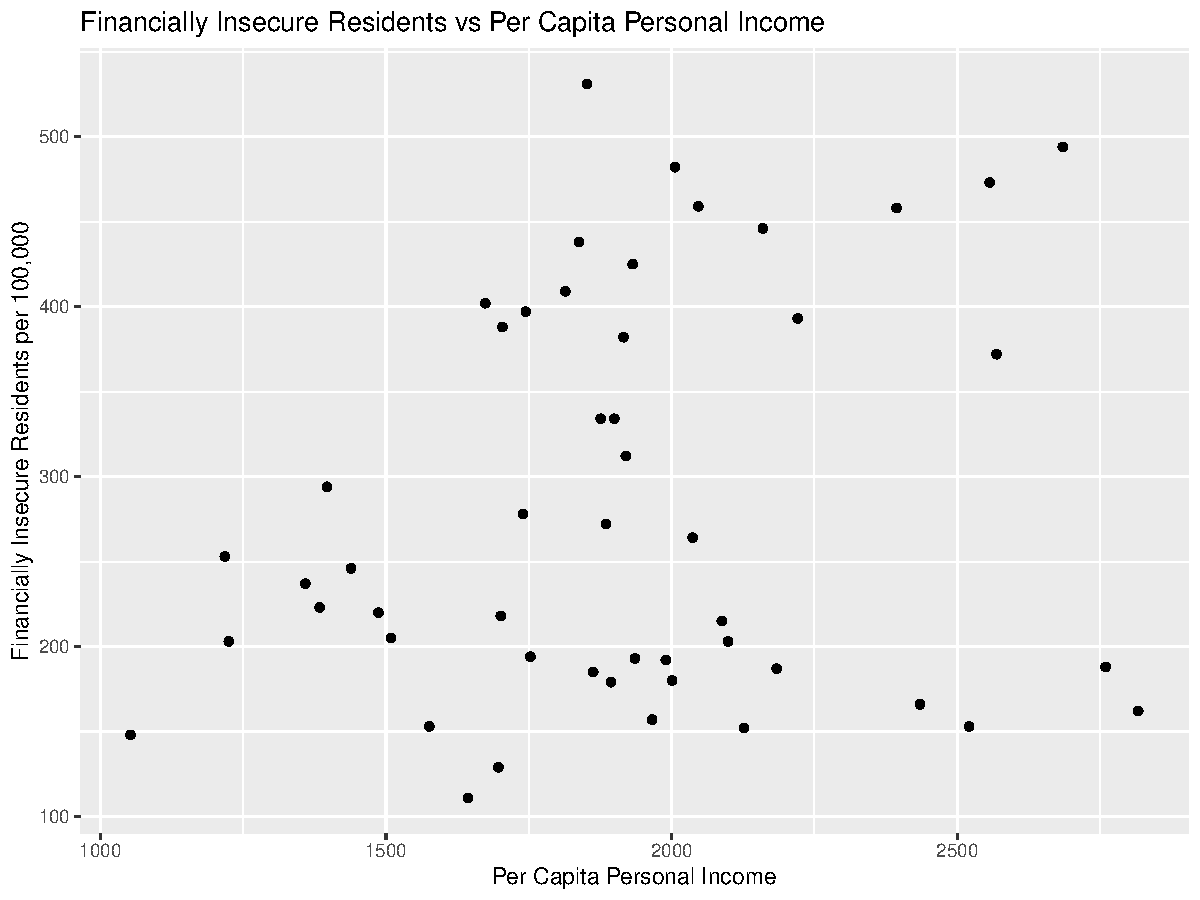
\includegraphics[width=.75\textwidth]{X1_X2.pdf}
\end{figure}

\begin{figure}[h!]\centering
	\caption{\footnotesize X1 X3}
	\label{fig:8}
	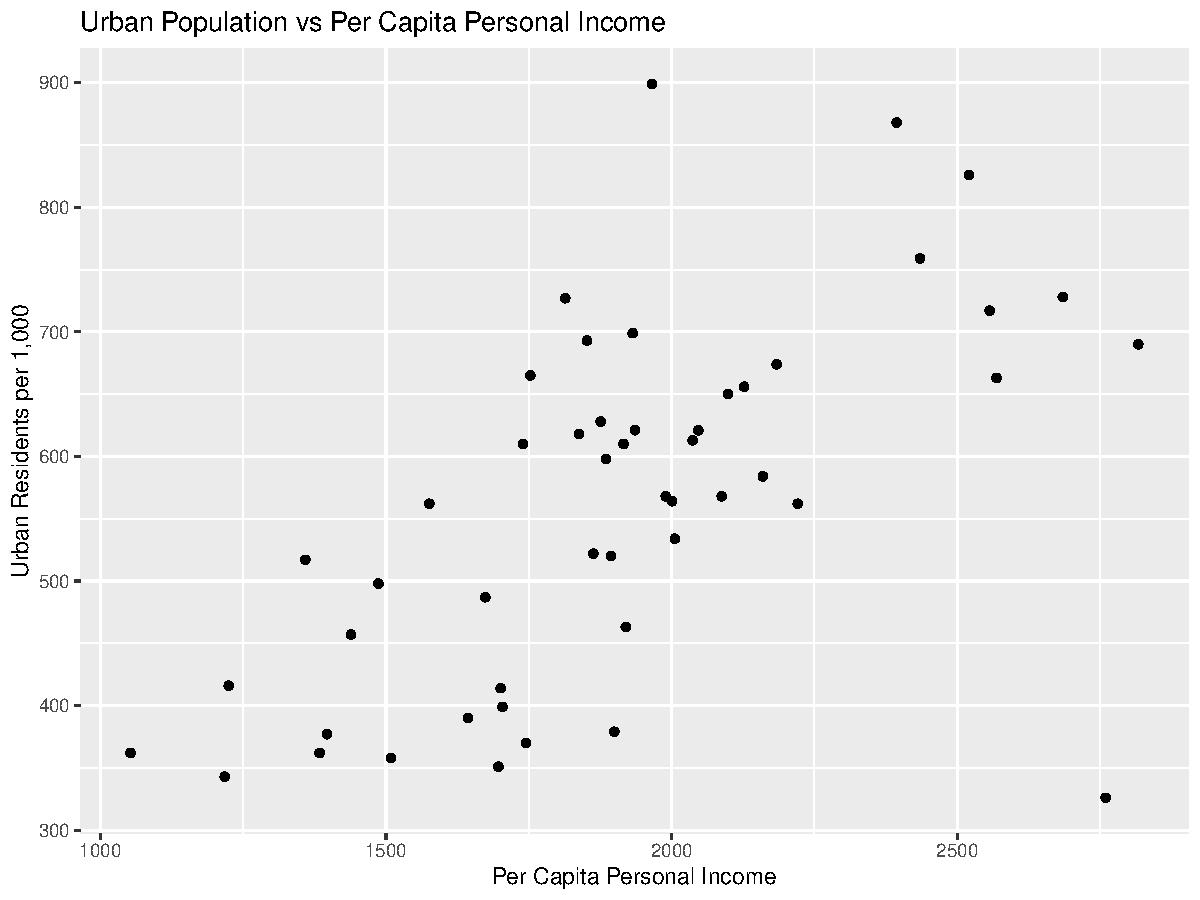
\includegraphics[width=.75\textwidth]{X1_X3.pdf}
\end{figure}

\begin{figure}[h!]\centering
	\caption{\footnotesize X2 X3}
	\label{fig:9}
	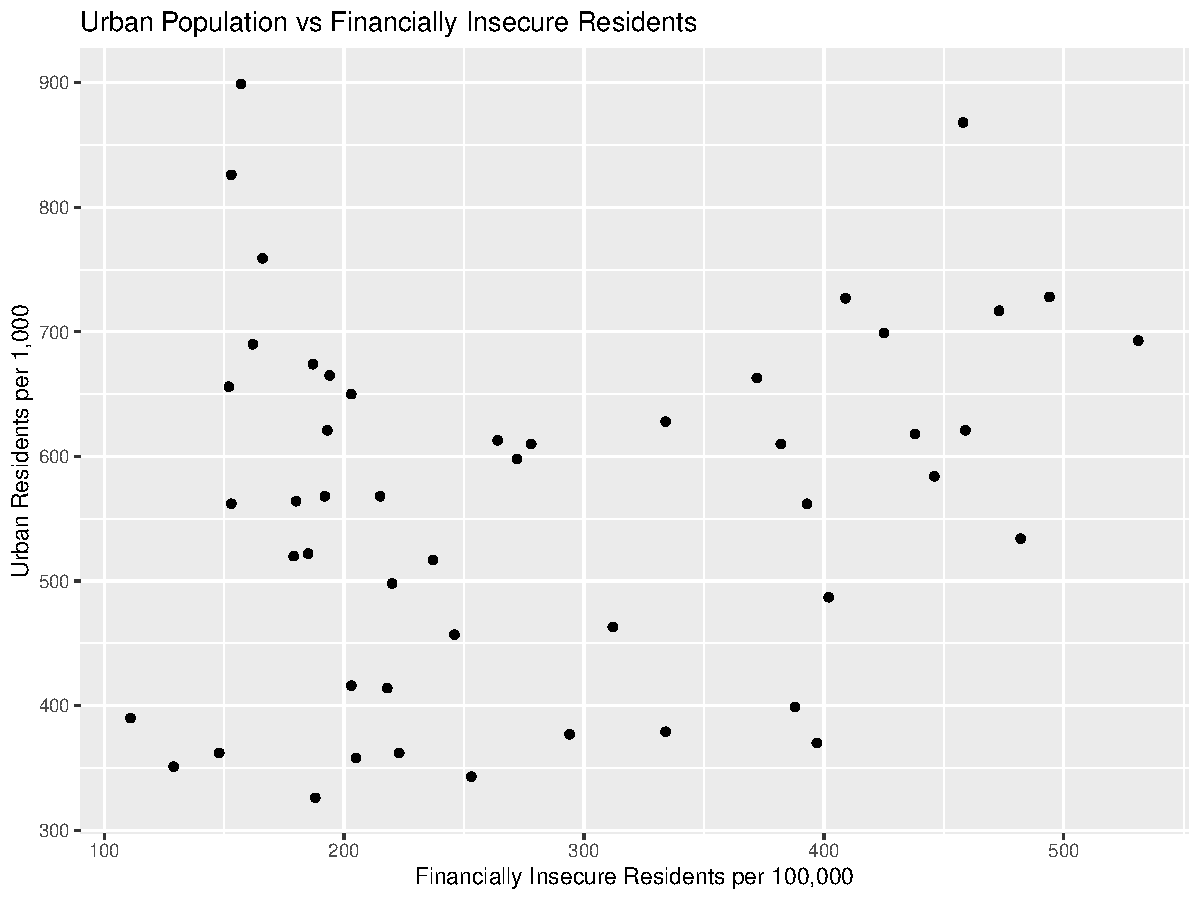
\includegraphics[width=.75\textwidth]{X2_X3.pdf}
\end{figure}

The scatter plots show a moderate positive relationship between per capita expenditure on housing assistance (Y) and each of the predictors: personal income (X1), financially insecure residents (X2), and urban population percentage (X3). This suggests that states with higher incomes, larger urban populations, and more financially vulnerable residents tend to spend more on addressing homelessness.\\

Please plot the relationship between \emph{Y} and \emph{Region}? On average, which region has the highest per capita expenditure on housing assistance?
\vspace{.2cm}
\lstinputlisting[language=R, firstline=122, lastline=130]{PS01.R} 

 \begin{figure}[h!]\centering
	\caption{\footnotesize Y Region}
	\label{fig:2}
	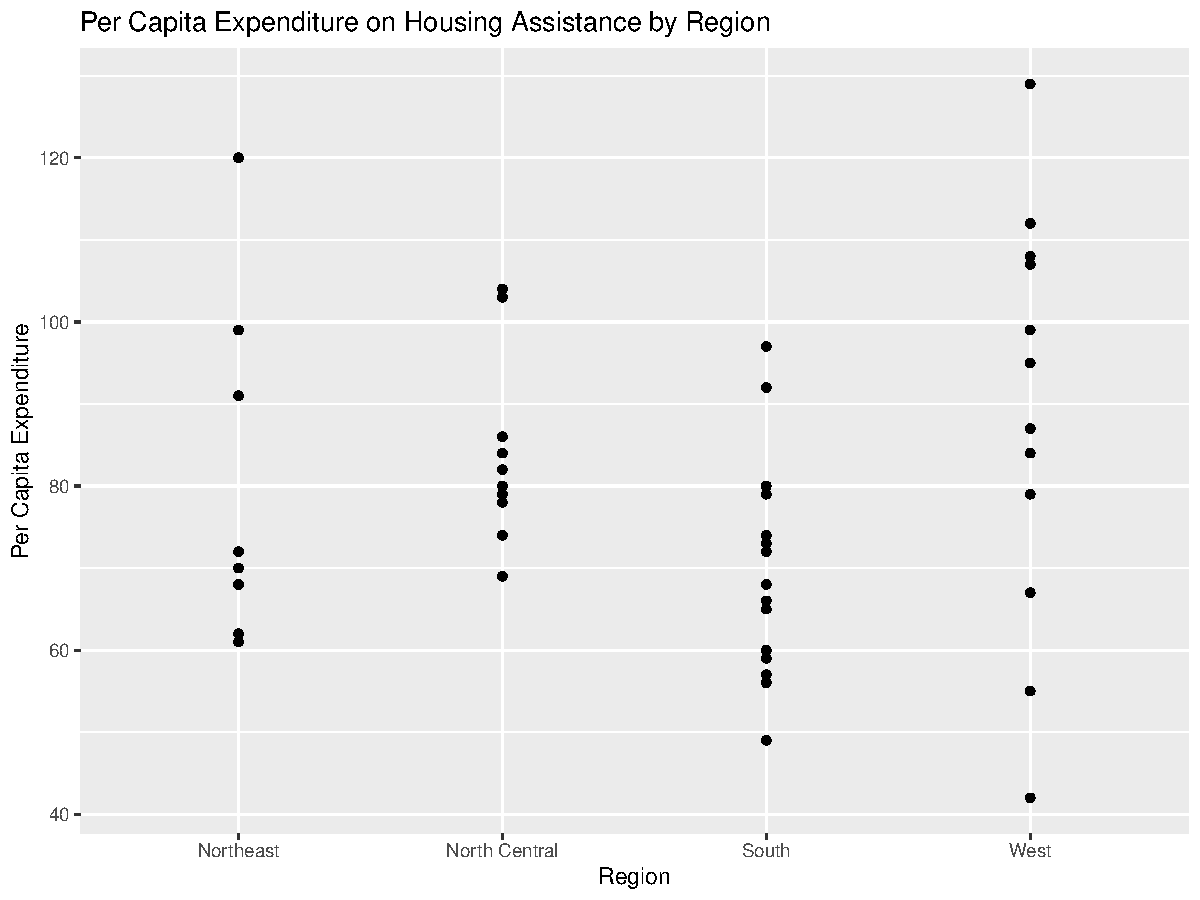
\includegraphics[width=.75\textwidth]{Y_VS_Region.pdf}
\end{figure}

Please plot the relationship between \emph{Y} and \emph{X1}? Describe this graph and the relationship. Reproduce the above graph including one more variable \emph{Region} and display different regions with different types of symbols and colors.
\vspace{.2cm}
\lstinputlisting[language=R, firstline=132, lastline=150]{PS01.R} 
\end{itemize}

 \begin{figure}[h!]\centering
	\caption{\footnotesize Y X1 Region}
	\label{fig:4}
	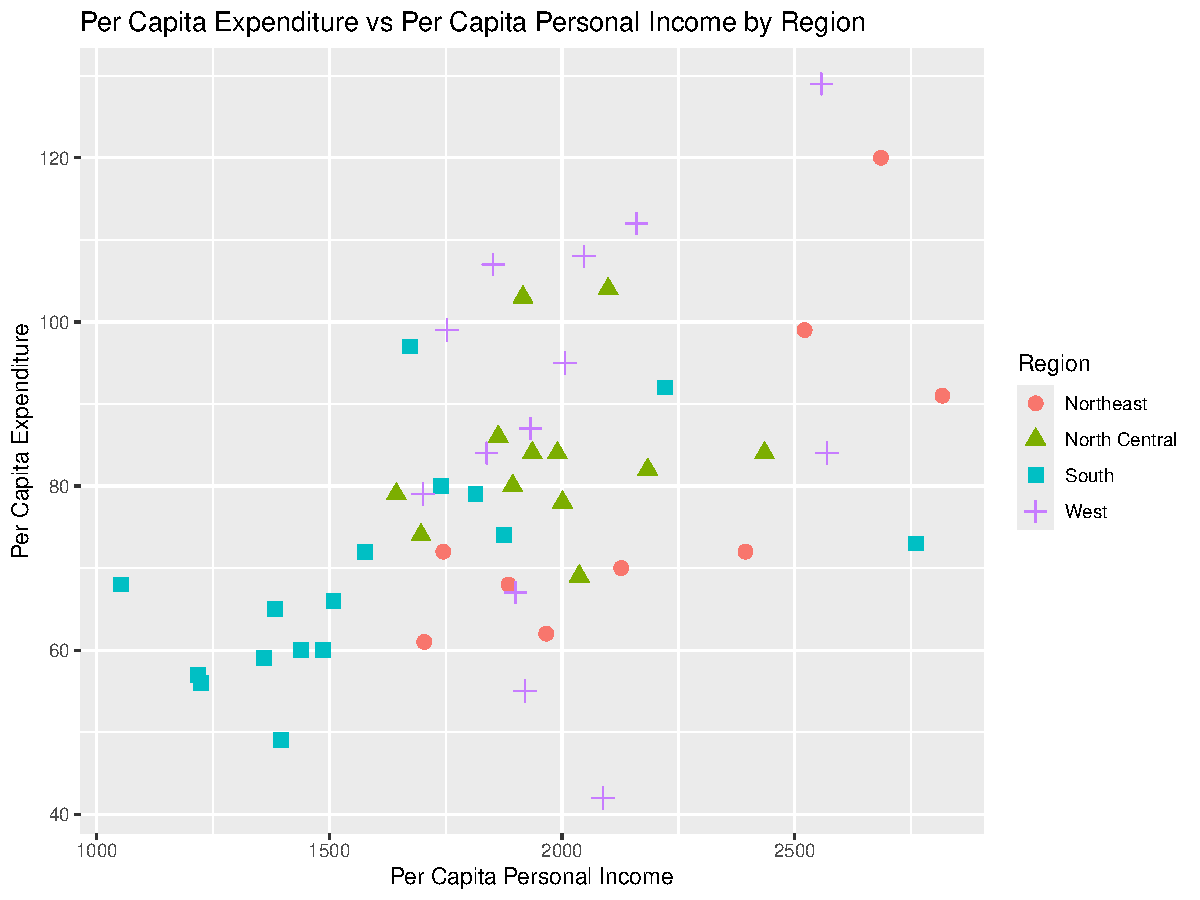
\includegraphics[width=.75\textwidth]{Y_X1_Region.pdf}
\end{figure}
The scatter plot of Y (per capita expenditure on housing assistance), X1 (personal income), and Region shows a positive relationship between Y and X1, with higher-income states spending more on housing assistance. However, regional differences are clear, with the Northeast and West regions generally spending more at similar income levels compared to the South and North Central. This suggests that both personal income and regional factors play significant roles in determining housing assistance expenditures.\\

\end{document}
